\documentclass[a4paper,twoside]{article}
\usepackage{blindtext}  
\usepackage{geometry}

% Chinese support
\usepackage[UTF8, scheme = plain]{ctex}

% Page margin layout
\geometry{left=2.3cm,right=2cm,top=2.5cm,bottom=2.0cm}


\usepackage{listings}
\usepackage{xcolor}
\usepackage{geometry}
\usepackage{amsmath}
\usepackage{float}
\usepackage{hyperref}

\usepackage{graphics}
\usepackage{graphicx}
\usepackage{epsfig}
\usepackage{float}

\usepackage{algorithm}
\usepackage[noend]{algpseudocode}

\usepackage{booktabs}
\usepackage{threeparttable}
\usepackage{longtable}
\usepackage{listings}
\usepackage{tikz}
\usepackage{multicol}

\usepackage{caption}
\usepackage{subcaption}

% cite package, to clean up citations in the main text. Do not remove.
\usepackage{cite}

\usepackage{color,xcolor}

%% The amssymb package provides various useful mathematical symbols
\usepackage{amssymb}
%% The amsthm package provides extended theorem environments
\usepackage{amsthm}
\usepackage{amsfonts}
\usepackage{enumerate}
\usepackage{enumitem}
\usepackage{listings}

\usepackage{indentfirst}
\setlength{\parindent}{2em} % Make two letter space in the first paragraph
\usepackage{setspace}
\linespread{1.5} % Line spacing setting
\usepackage{siunitx}
\setlength{\parskip}{0.5em} % Paragraph spacing setting

% \usepackage[contents =22920202204622, scale = 10, color = black, angle = 50, opacity = .10]{background}

\renewcommand{\figurename}{图}
\renewcommand{\lstlistingname}{代码} 
\renewcommand{\tablename}{表格}
\renewcommand{\contentsname}{目录}
\floatname{algorithm}{算法}

\graphicspath{ {images/} }

%%%%%%%%%%%%%
\newcommand{\StudentNumber}{22920202204622}  % Fill your student number here
\newcommand{\StudentName}{熊恪峥}  % Replace your name here
\newcommand{\PaperTitle}{实验(二)}  % Change your paper title here
\newcommand{\PaperType}{实验报告} % Replace the type of your report here
\newcommand{\Date}{2022年10月18日}
\newcommand{\College}{信息学院}
\newcommand{\CourseName}{计算机网络}
%%%%%%%%%%%%%

%% Page header and footer setting
\usepackage{fancyhdr}
\usepackage{lastpage}
\pagestyle{fancy}
\fancyhf{}
% This requires the document to be twoside
\fancyhead[LO]{\texttt{\StudentName }}
\fancyhead[LE]{\texttt{\StudentNumber}}
\fancyhead[C]{\texttt{\PaperTitle }}
\fancyhead[R]{\texttt{第{\thepage}页,共\pageref*{LastPage}页}}


\title{\PaperTitle}
\author{\StudentName}
\date{\Date}

\lstset{
	basicstyle          =   \sffamily,          % 基本代码风格
	keywordstyle        =   \bfseries,          % 关键字风格
	commentstyle        =   \rmfamily\itshape,  % 注释的风格,斜体
	stringstyle         =   \ttfamily,  % 字符串风格
	flexiblecolumns,                % 别问为什么,加上这个
	numbers             =   left,   % 行号的位置在左边
	showspaces          =   false,  % 是否显示空格,显示了有点乱,所以不现实了
	numberstyle         =   \zihao{-5}\ttfamily,    % 行号的样式,小五号,tt等宽字体
	showstringspaces    =   false,
	captionpos          =   t,      % 这段代码的名字所呈现的位置,t指的是top上面
	frame               =   lrtb,   % 显示边框
}

\lstdefinestyle{PythonStyle}{
	language        =   Python, % 语言选Python
	basicstyle      =   \zihao{-5}\ttfamily,
	numberstyle     =   \zihao{-5}\ttfamily,
	keywordstyle    =   \color{blue},
	keywordstyle    =   [2] \color{teal},
	stringstyle     =   \color{magenta},
	commentstyle    =   \color{red}\ttfamily,
	breaklines      =   true,   % 自动换行,建议不要写太长的行
	columns         =   fixed,  % 如果不加这一句,字间距就不固定,很丑,必须加
	basewidth       =   0.5em,
}

\lstdefinestyle{MakefileStyle}{
	otherkeywords={.SUFFIXES},
	morekeywords={SUFFIX, CPP_,},
	moredelim=[is][\color{mbleu}]{/*}{*/},
	morecomment=[l][commentstyle]{\#},%
	emphstyle={\color{teal}},%
	moredelim=[s][\color{teal}]{\$(}{)}%
	basicstyle=\ttfamily\scriptsize\color{black!90},%
	stringstyle=\itshape\color{magenta},%
	showstringspaces=false,%
	keywordstyle=\bfseries\color{keycolor},%
	commentstyle=\color{blue}\slshape,%
	framexleftmargin=1mm,%
	backgroundcolor=\color{black!2},%
}

\lstdefinestyle{CppStyle}{
	language        =   c++,
	basicstyle      =   \zihao{-5}\ttfamily,
	numberstyle     =   \zihao{-5}\ttfamily,
	keywordstyle    =   \color{blue},
	keywordstyle    =   [2] \color{teal},
	stringstyle     =   \color{magenta},
	commentstyle    =   \color{red}\ttfamily,
	breaklines      =   true,   % 自动换行,建议不要写太长的行
	columns         =   fixed,  % 如果不加这一句,字间距就不固定,很丑,必须加
	basewidth       =   0.5em,
}

\algnewcommand\algorithmicinput{\textbf{Input:}}
\algnewcommand\algorithmicoutput{\textbf{Output:}}
\algnewcommand\Input{\item[\algorithmicinput]}%
\algnewcommand\Output{\item[\algorithmicoutput]}%

\usetikzlibrary{positioning, shapes.geometric}

% 流程图定义基本形状
\tikzstyle{startstop} = [rectangle, rounded corners, minimum width = 2cm, minimum height=1cm,text centered, draw = black]
\tikzstyle{io} = [trapezium, trapezium left angle=70, trapezium right angle=110, minimum width=2cm, minimum height=1cm, text centered, draw=black]
\tikzstyle{process} = [rectangle, minimum width=3cm, minimum height=1cm, text centered, draw=black]
\tikzstyle{decision} = [diamond, aspect = 3, text centered, draw=black]
% 箭头形式
\tikzstyle{arrow} = [->,>=stealth]

\newtheorem{assumption}{Assumption}[section]

\begin{document}
	
%%%%%%%%%%%%%%%%%%%%%%%%%%%%%%%%%%%%%%%%%%%%
\makeatletter % change default title style
\renewcommand*\maketitle{%
	\begin{center} 
		\bfseries  % title 
		{\LARGE \@title \par}  % LARGE typesetting
		\vskip 1em  %  margin 1em
		{\global\let\author\@empty}  % no author information
		{\global\let\date\@empty}  % no date
		\thispagestyle{empty}   %  empty page style
	\end{center}%
	\setcounter{footnote}{0}%
}
\makeatother
%%%%%%%%%%%%%%%%%%%%%%%%%%%%%%%%%%%%%%%%%%%%
	
	
\thispagestyle{empty}

\vspace*{1cm}

\begin{figure}[h]
	\centering
	
\includegraphics[width=4.0cm]{logo.png}
\end{figure}

\vspace*{1cm}

\begin{center}
	\Huge{\textbf{\PaperType}}
	
	\Large{\PaperTitle}
\end{center}

\vspace*{1cm}

\begin{table}[h]
	\centering	
	\begin{Large}
		\renewcommand{\arraystretch}{1.5}
		\begin{tabular}{p{3cm} p{5cm}<{\centering}}
			姓\qquad 名 & \StudentName  \\
			\hline
			学\qquad号 & \StudentNumber \\
			\hline
			日\qquad期 & \Date  \\
			\hline
			学\qquad院 & \College  \\
			\hline
			课程名称 & \CourseName  \\
			\hline
		\end{tabular}
	\end{Large}
\end{table}

\newpage

\title{
	\Large{\textcolor{black}{\PaperTitle}}
}
	
	
\maketitle
	
\tableofcontents
 
\newpage
\setcounter{page}{1}

\begin{spacing}{1.2}

\section{捕获和分析有线以太网数据包}

\subsection{分析MAC帧}

首先在Wireshark中查看帧内容如图~\ref{fig:mac}

\begin{figure}[htb]
	\centering
	\caption{MAC帧内容}
	\label{fig:mac}
	\begin{subfigure}{0.4\textwidth}
		\centering
		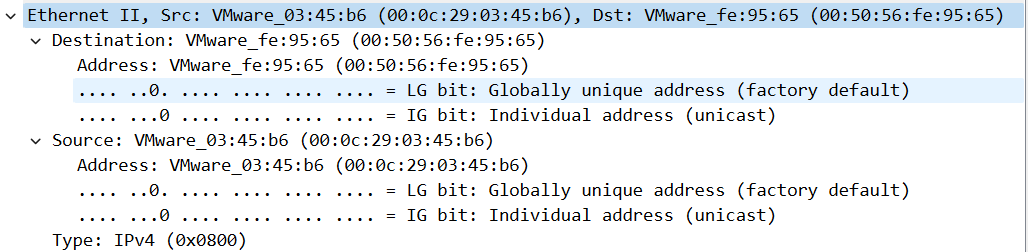
\includegraphics[width=\textwidth]{mac.png}
		\caption{内容}
		\label{fig:mac_det}
	\end{subfigure}
	\begin{subfigure}{0.4\textwidth}
		\centering
		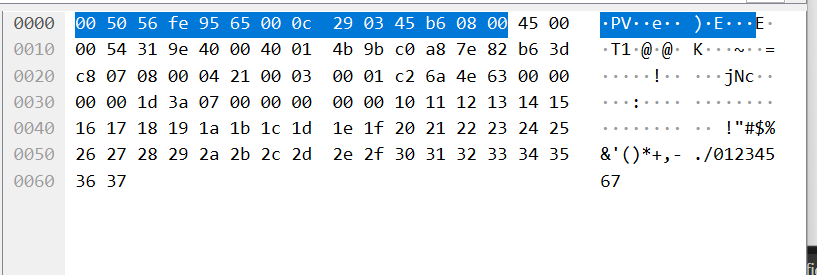
\includegraphics[width=\textwidth]{mac_raw.png}
		\caption{原始数据}
		\label{fig:mac_raw}
	\end{subfigure}
\end{figure}

根据MAC帧格式,前12字节分别是目的地址和源地址。因此目的地址是
$00:50:56:fe:95:95$,源地址是$00:0c:29:03:45:b6$。
类型字段的值是$0x0800$,表示下一层是IP协议。

EUI-48地址,也就是MAC地址,是一个48位的二进制数。它的前24位是厂商的OUI。
其中第一个字节的后两位分别表示了是否是全局唯一的地址和是否是多播地址。
例如目的地址的前两位是$00$,表示是全局唯一的地址,进行单播;源地址也是如此。


\subsection{分析IP数据报首部}

IP数据报的内容如图~\ref{fig:ip}。

\begin{figure}[htb]
	\centering
	\caption{IP数据报}
	\label{fig:ip}
	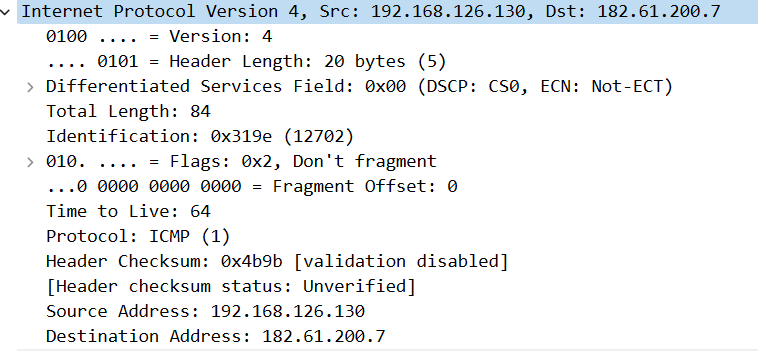
\includegraphics[width=0.6\textwidth]{ip.png}
\end{figure}

前4位为版本号,说明这个报文是IPv4;其后4位是首部长度,本报首部长度为20字节;
然后是区分服务(Differentiated services)DS,占1字节。
IP报总长度,占4位,本数据报总长度为84字节。然后是标识,占16位;
之后是标志,占3位,有禁止分段的标志。然后是偏移,占13位,本请求帧没有分片,所以片偏移量为0;
生存时间,占8位,表明数据报在互联网中至多可经过多少个路由器。本数据报TTL为64;
然后是协议字段,占8位,表明此数据报携带的数据是使用何种协议,本数据报使用ICMP
之后是首部检验和,占16位。最后源地址和目的地址各占32位。

帧长比数据报长要长,因为在不同的层会加入额外的首部。

\subsection{观察IP分片}

根据实验内容,(a)是普通的ping请求。(b)、(c)、(d)用不同长度的数据包进行ping请求。
其中(b)、(c)发送了禁止分段标记,(c)、(d)形成的数据长度超过了MTU,因此ping的效果
如图~\ref{fig:ip_frag}所示。


\begin{figure}[htb]
	\centering
	\caption{Ping结果}
	\label{fig:ip_frag}
	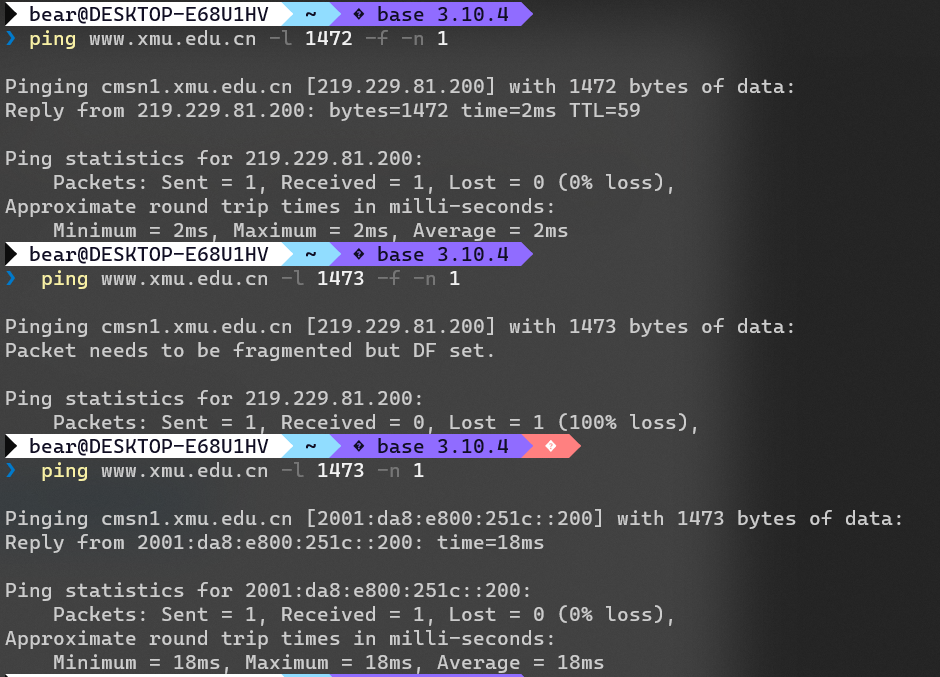
\includegraphics[width=0.6\textwidth]{ip_frag.png}
\end{figure}

可见,(c)无法成功,因为应当分片,但由于禁止分片标记而不能分段,因此无法成功。

观察数据包的长度,如图~\ref{fig:frag_len},发现当包长度超过1472时ICMP请求变短了。
改变过滤条件,发现出现了IP分片数据报,如图~\ref{fig:frag_detail}所示。
因此,当数据变长时会产生分片。这里测试了1473、1479两种长度,可以发现
分片的所有数据报长度之和是正常的。


\begin{figure}[htb]
	\centering
	\caption{分片数据报}
	\label{fig:frag}
	\begin{subfigure}{0.4\textwidth}
		\centering
		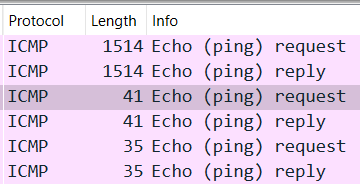
\includegraphics[width=\textwidth]{frag_len.png}
		\caption{长度}
		\label{fig:frag_len}
	\end{subfigure}
	\begin{subfigure}{0.4\textwidth}
		\centering
		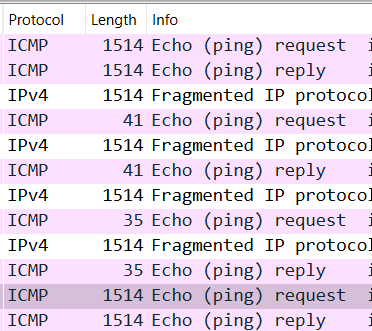
\includegraphics[width=\textwidth]{frag.png}
		\caption{分片数据报}
		\label{fig:frag_detail}
	\end{subfigure}
\end{figure}

\subsection{ICMP协议分析}

在Windows下,一次Ping命令会进行4次ICMP请求,因此有8个数据报,其中四次请求四次回应。如图~\ref{fig:icmp}所示。

\begin{figure}[htb]
	\centering
	\caption{Ping产生的数据报}
	\label{fig:icmp}
	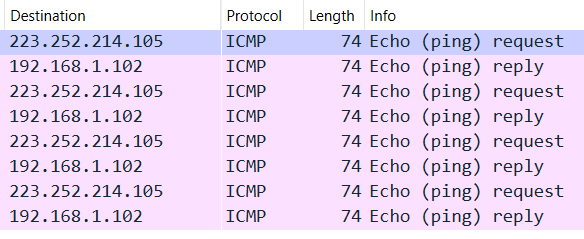
\includegraphics[width=0.6\textwidth]{icmp.png}
\end{figure}

数据包内容如图~\ref{fig:icmp_detail},ICMP请求和回应的Code分别为8-0和0-0。
IP部分首先两者的源地址和目的地址相反,其次TTL也不一样,可能是由于操作系统不同。

\begin{figure}[htb]
	\centering
	\caption{ICMP请求}
	\label{fig:icmp_detail}
	\begin{subfigure}{0.4\textwidth}
		\centering
		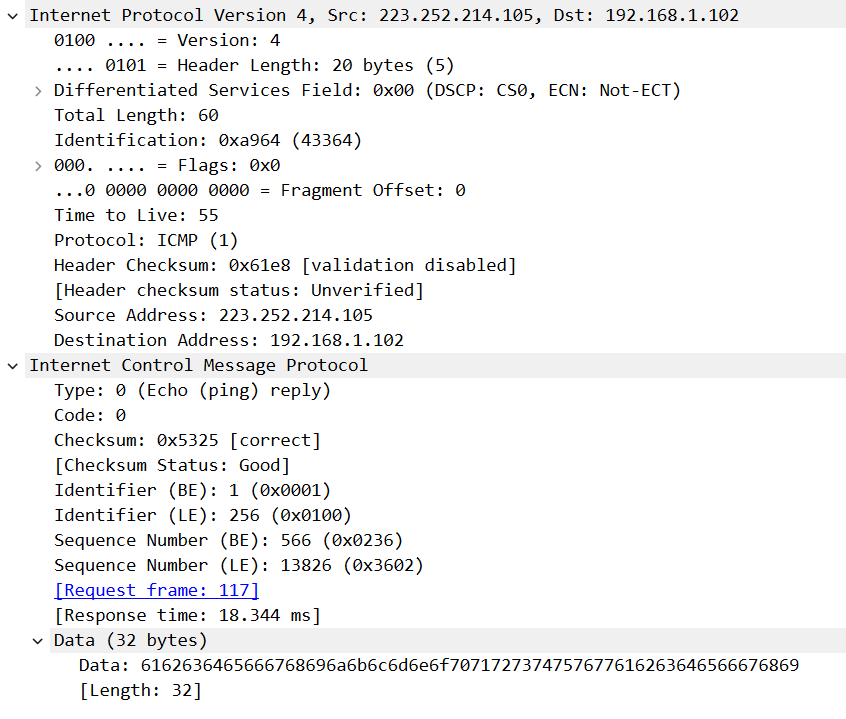
\includegraphics[width=\textwidth]{icmp_req.png}
		\caption{请求}
		\label{fig:icmp_req}
	\end{subfigure}
	\begin{subfigure}{0.4\textwidth}
		\centering
		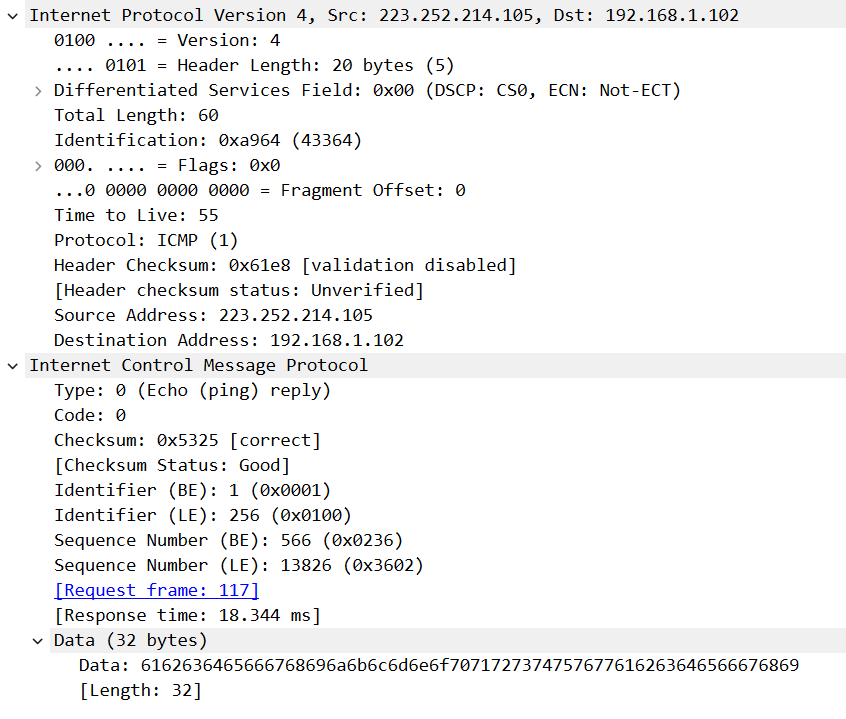
\includegraphics[width=\textwidth]{icmp_req.png}
		\caption{回复}
		\label{fig:icmp_rep}
	\end{subfigure}
\end{figure}

\subsection{tracert工作原理分析}

tracert程序的设计利用ICMP及TTL来列出所有经过的节点。

首先,tracert送出一个TTL是1的数据报到目的地,
当路径上的第一个路由器收到时,它将TTL减1。此时,TTL变为0,所以该路由器会将数据报丢掉,
并送回一个ICMP包,这包括发IP包的源地址,IP包的所有内容及路由器的IP地址,tracert收到这个消息后便知道这个路由器存在于这个路径上,
接着tracert再送出另一个TTL是2的数据报,以此类推,traceroute每次将送出的数据报的TTL加1来发现下一个路由器,
这个重复的动作一直持续到某个数据报抵达目的地。这时,该主机并不会送回ICMP消息,因为它已是目的地了。

过程大致如图~\ref{fig:tracert_ill}。

\begin{figure}[htb]
	\centering
	\caption{tracert原理}
	\label{fig:tracert_ill}
	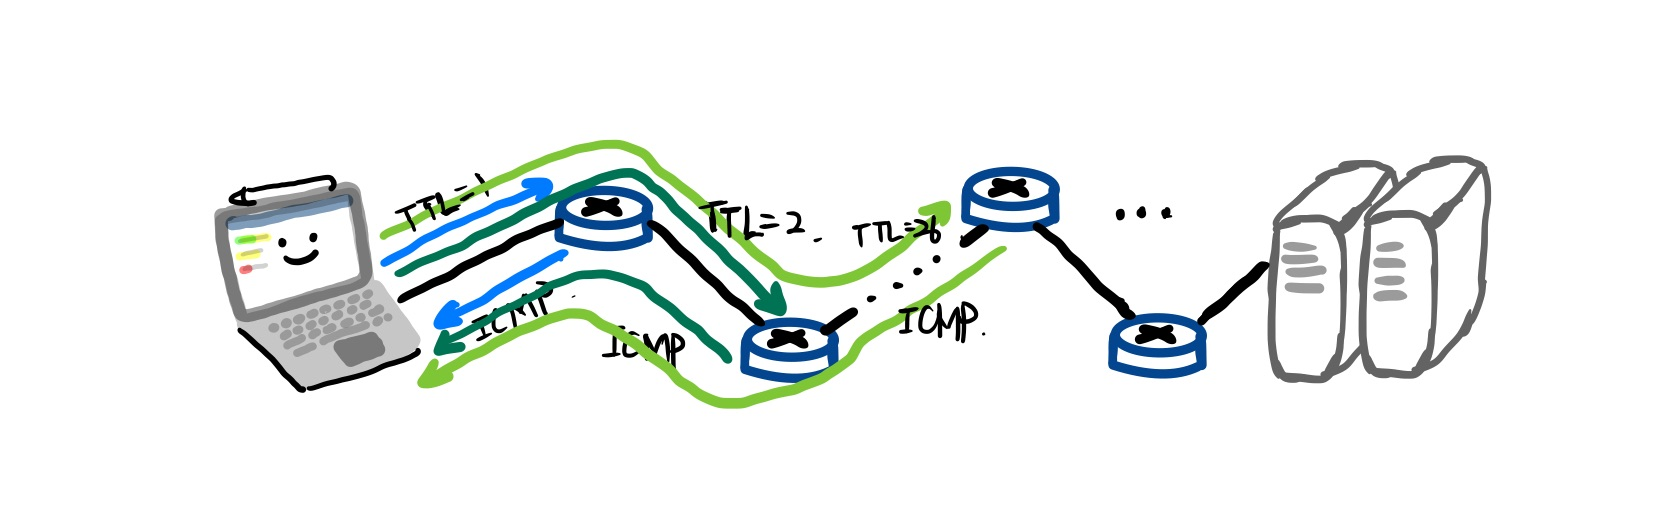
\includegraphics[width=0.8\textwidth]{tracert_method.png}
\end{figure}


图~\ref{fig:tracert}是使用tracert跟踪GitHub的结果。可以看到,tracert会发送多个数据报,每个数据报的TTL不同,这样就可以跟踪到路径上的所有节点。
到达GitHub需要28跳,因为服务器在美国,所以需要经过很多跳的路由器。因此这个结果符合实际情况。

\begin{figure}[htb]
	\centering
	\caption{tracert}
	\label{fig:tracert}
	\begin{subfigure}{0.4\textwidth}
		\centering
		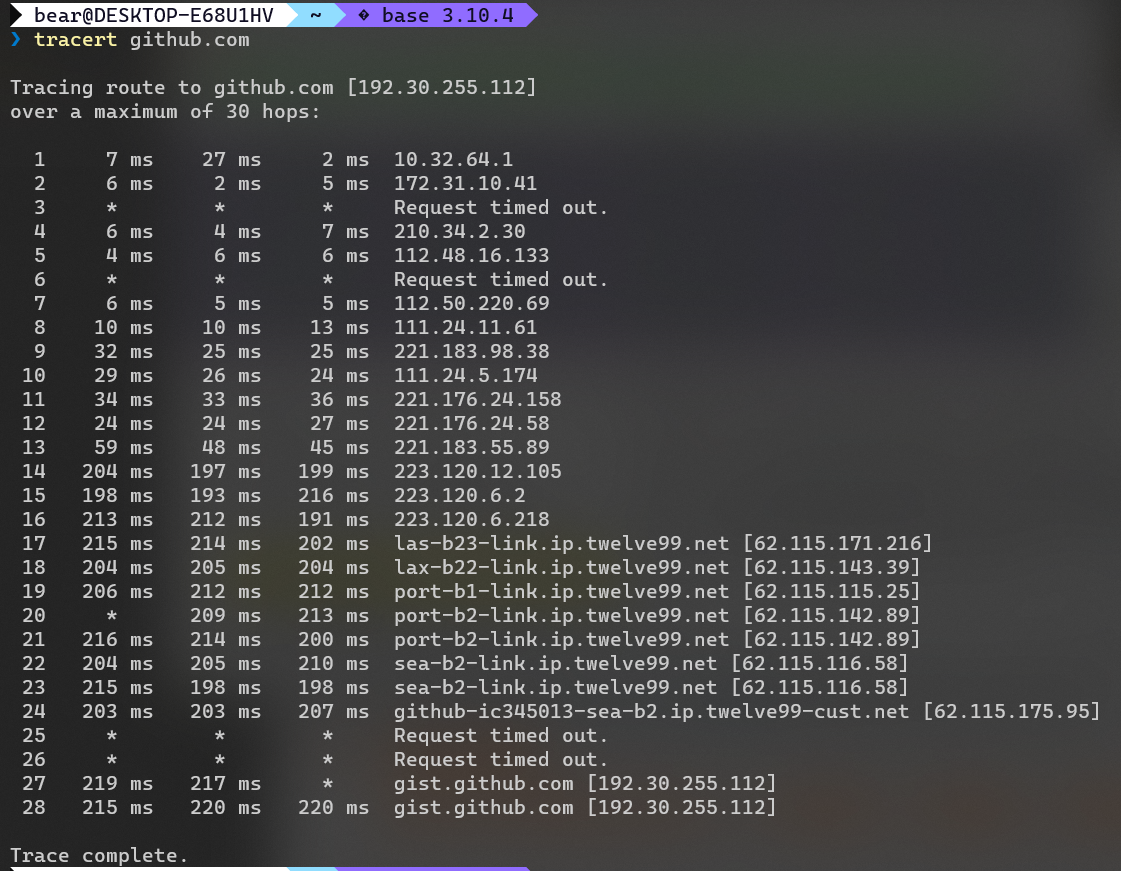
\includegraphics[width=\textwidth]{tracert.png}
		\caption{tracert输出}
		\label{fig:tracert_out}
	\end{subfigure}
	\begin{subfigure}{0.4\textwidth}
		\centering
		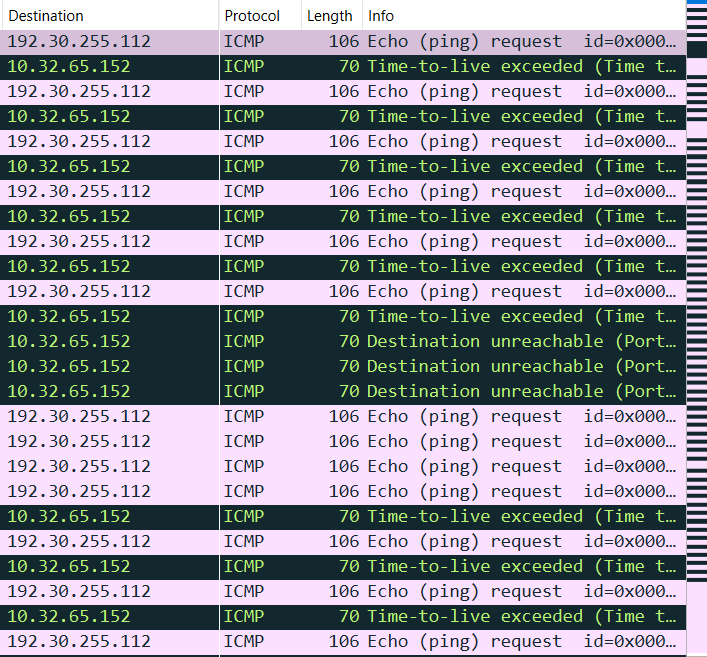
\includegraphics[width=\textwidth]{tracert_package.png}
		\caption{产生的数据报}
		\label{fig:tracert_pack}
	\end{subfigure}
\end{figure}

\subsection{ARP协议分析}

实验要求ping到局域网内的主机和远程主机,分析数据包内容。由于使用WIFI时不能保证两人
一定在同一局域网中,因此我使用了另一种方法。

当虚拟机网络模式为NAT时,虚拟机和宿主机可以认为是在同一局域网中的主机,因此从
虚拟机Ping宿主机的时候可以得到和Ping局域网内的主机一样的效果。如图~\ref{fig:arp}

\begin{figure}[H]
	\centering
	\caption{ARP请求}
	\label{fig:arp}
	\begin{subfigure}{0.4\textwidth}
		\centering
		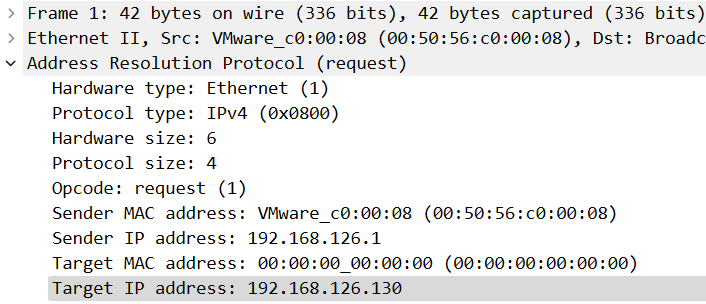
\includegraphics[width=\textwidth]{arp_req.png}
		\caption{请求}
		\label{fig:arp_req}
	\end{subfigure}
	\begin{subfigure}{0.4\textwidth}
		\centering
		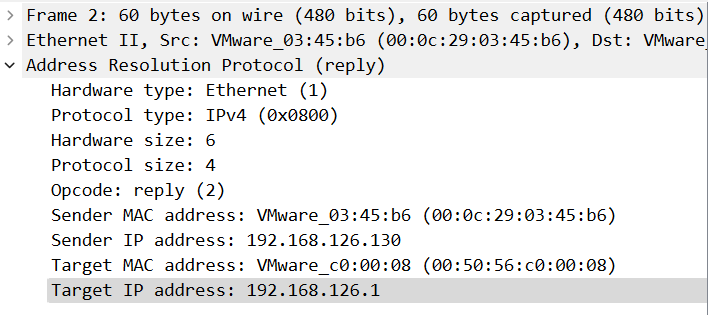
\includegraphics[width=\textwidth]{arp_rep.png}
		\caption{回复}
		\label{fig:arp_rep}
	\end{subfigure}
\end{figure}

ARP请求如图~\ref{fig:arp_req},其中目的MAC地址是0,说明在进行广播。
此时,位于192.168.126.130的虚拟机收到了ARP请求,并进行了回复,如图~\ref{fig:arp_rep}。
这样就知道了虚拟机的MAC地址。然后会加入ARP表中。

而Ping远程主机时则会产生对网关的ARP请求,如图~\ref{fig:arp_rem}。

\begin{figure}[H]
	\centering
	\caption{Ping远程主机产生的ARP}
	\label{fig:arp_rem}
	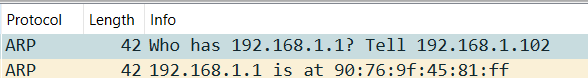
\includegraphics[width=0.6\textwidth]{arp_remote.png}
\end{figure}

因为根据ARP的工作方式,所有帧都必须传送到本地网段中的节点。 如果目的 IPv4 主机在本地网络上,帧将使用此设备的 MAC 地址作为目的 MAC 地址。
如果目的 IPv4 主机不在本地网络上,则源节点需要将帧传送到作为网关的路由器接口,或用于到达该目的地的下一跳。 
源节点将使用网关的 MAC 地址作为帧(其中含有发往其它网络上主机的 IPv4 数据包)的目的地址。
因此会产生这种现象。

\section{捕获和分析802.11数据}

在按照实验要求进行实验时,需要注意:在Linux中启动Wireshark需要root权限。否则无法访问虚拟网卡。

\subsection{管理帧}

在抓到的包中可以发现Probe Request和Beacon两种管理帧。如图~\ref{fig:ctl}。
Beacon帧主要来声明网络的存在。定期传送的信标可让移动式工作站该网络的存在,从而调整加入该网络所必需的参数。
设备通过Probe Request帧来扫描所在区域内的802.11网络。 若Probe Request帧探查的网络与之兼容,该网络就会回复Probe Response帧给予响应。

其中Beacon帧广播了SSID、信道、BSSID等信息,如图~\ref{fig:beacon}。

可以看出SSID是XMUNET+,信道是1,BSSID是d0:15:a6:43:eb:81。

\begin{figure}[H]
	\centering
	\caption{管理帧}
	\label{fig:ctl}
	\begin{subfigure}{0.4\textwidth}
		\centering
		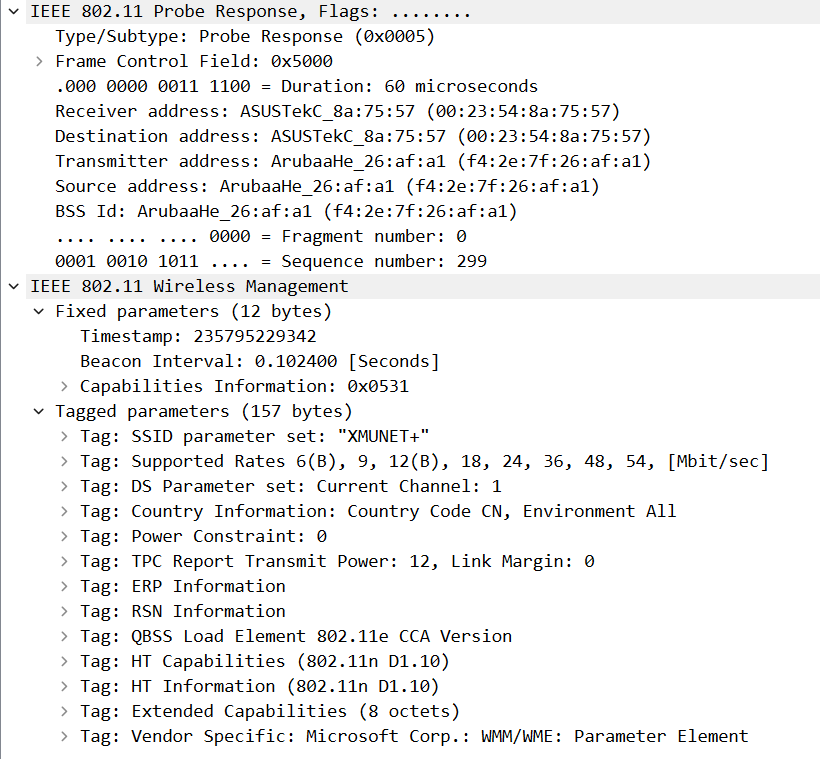
\includegraphics[width=\textwidth]{prob_res.png}
		\caption{Probe Response}
		\label{fig:prob_res}
	\end{subfigure}
	\begin{subfigure}{0.4\textwidth}
		\centering
		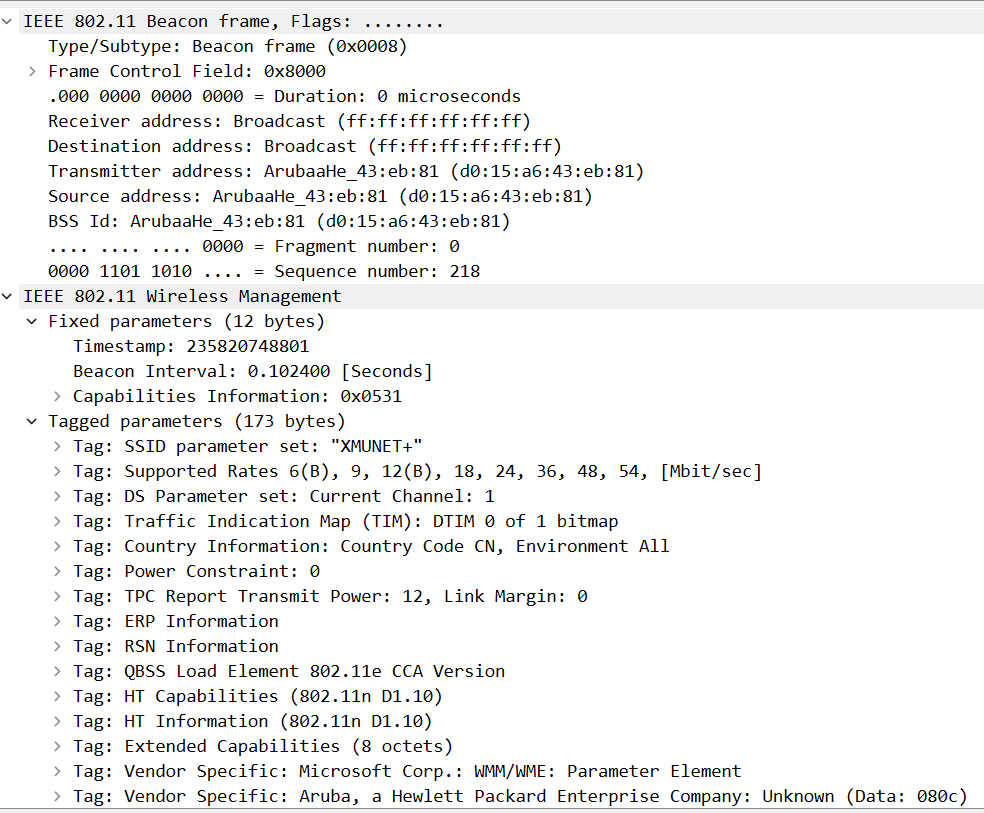
\includegraphics[width=\textwidth]{beacon.png}
		\caption{Beacon}
		\label{fig:beacon}
	\end{subfigure}
\end{figure}


\subsection{数据帧}

在抓到的包中可以发现Data、NULL Data、QoS Data和NULL QoS Data4种数据帧。如图~\ref{fig:dt}。

数据帧会将上层协议的数据置于帧主体加以传递。

\begin{figure}[H]
	\centering
	\caption{数据帧}
	\label{fig:dt}
	\begin{subfigure}{0.4\textwidth}
		\centering
		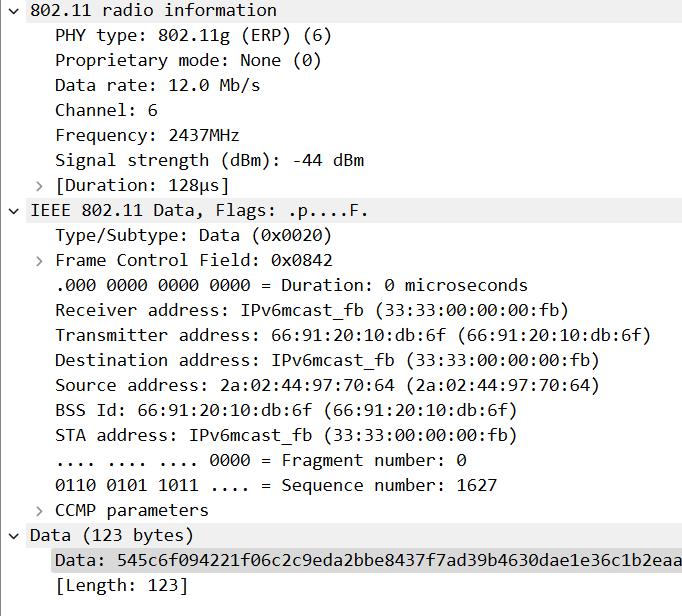
\includegraphics[width=\textwidth]{data.png}
		\caption{Data}
		\label{fig:data}
	\end{subfigure}
	\begin{subfigure}{0.4\textwidth}
		\centering
		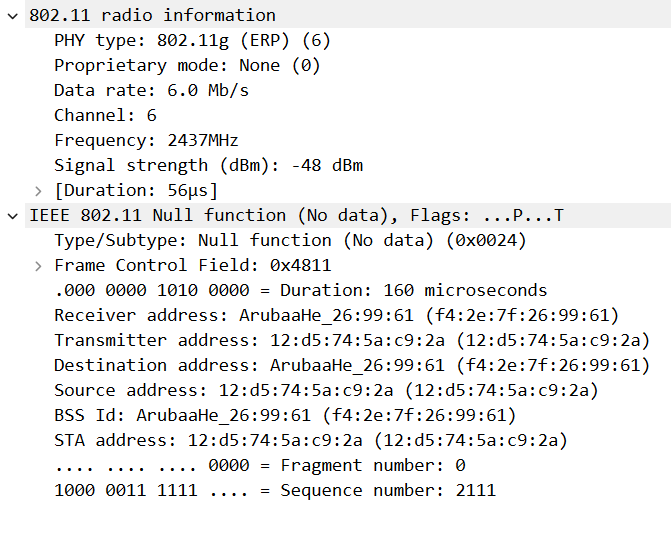
\includegraphics[width=\textwidth]{nf.png}
		\caption{Null Function}
		\label{fig:nf}
	\end{subfigure}
	\begin{subfigure}{0.4\textwidth}
		\centering
		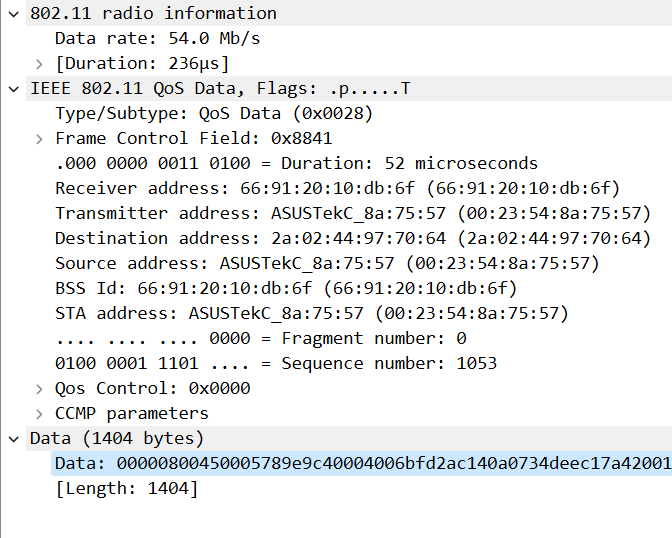
\includegraphics[width=\textwidth]{qos_data.png}
		\caption{QOS Data}
		\label{fig:qd}
	\end{subfigure}
	\begin{subfigure}{0.4\textwidth}
		\centering
		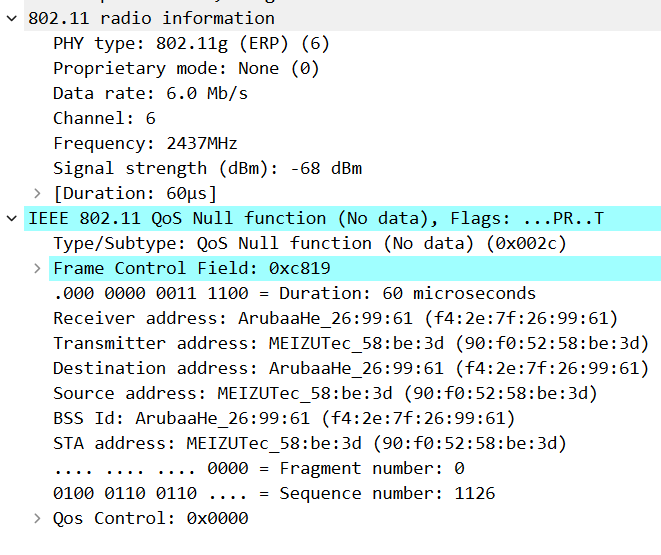
\includegraphics[width=\textwidth]{qos_nf.png}
		\caption{QOS Null Function}
		\label{fig:qnf}
	\end{subfigure}
\end{figure}


\subsection{控制帧}

在抓到的包中可以发现Acknowledgment和Clear to Send两种控制帧。如图~\ref{fig:mng}。
每个发送的单播报文,接收者在成功接收到发送报文后,都要发送一个应答ACK进行确认。
它的Duration是8微秒,能够反映出ACK 信号在整个帧交换过程中位居何处。

目的客户端收到RTS后,发送一个CTS报文,这样在客户端覆盖范围内所有的设备都会在指定的时间内不发送数据。
这里指定的时间是3805微秒。

\begin{figure}[H]
	\centering
	\caption{控制帧}
	\label{fig:mng}
	\begin{subfigure}{0.4\textwidth}
		\centering
		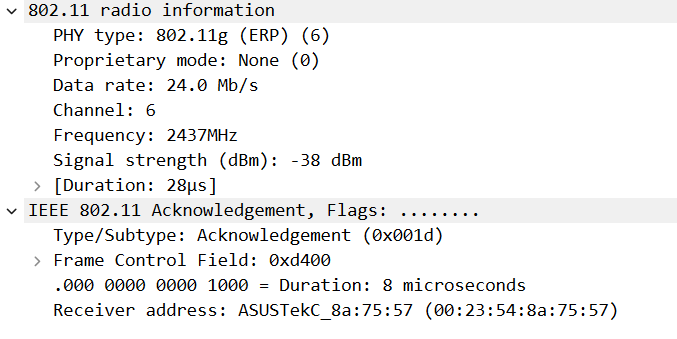
\includegraphics[width=\textwidth]{ack.png}
		\caption{Acknowledgment}
		\label{fig:ack}
	\end{subfigure}
	\begin{subfigure}{0.4\textwidth}
		\centering
		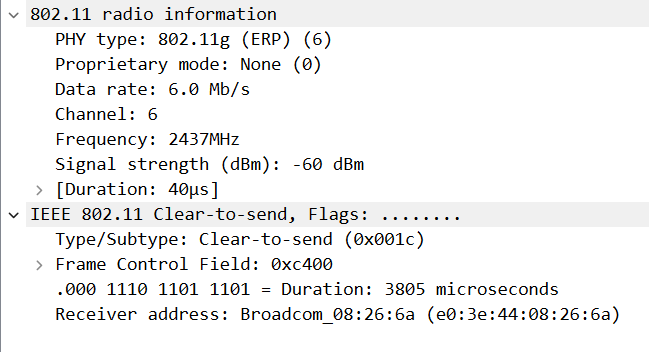
\includegraphics[width=\textwidth]{cts.png}
		\caption{Clear to Send}
		\label{fig:cts}
	\end{subfigure}
\end{figure}


\clearpage
\section{探索Wireshark更多功能和其它抓包工具}

\subsection{数据流追踪}

向百度图片搜索发送图片,可以使用数据流追踪来追踪数据流的传输过程。如图~\ref{fig:dt_tr}。

\begin{figure}[htb]
	\centering
	\caption{数据流追踪}
	\label{fig:dt_tr}
	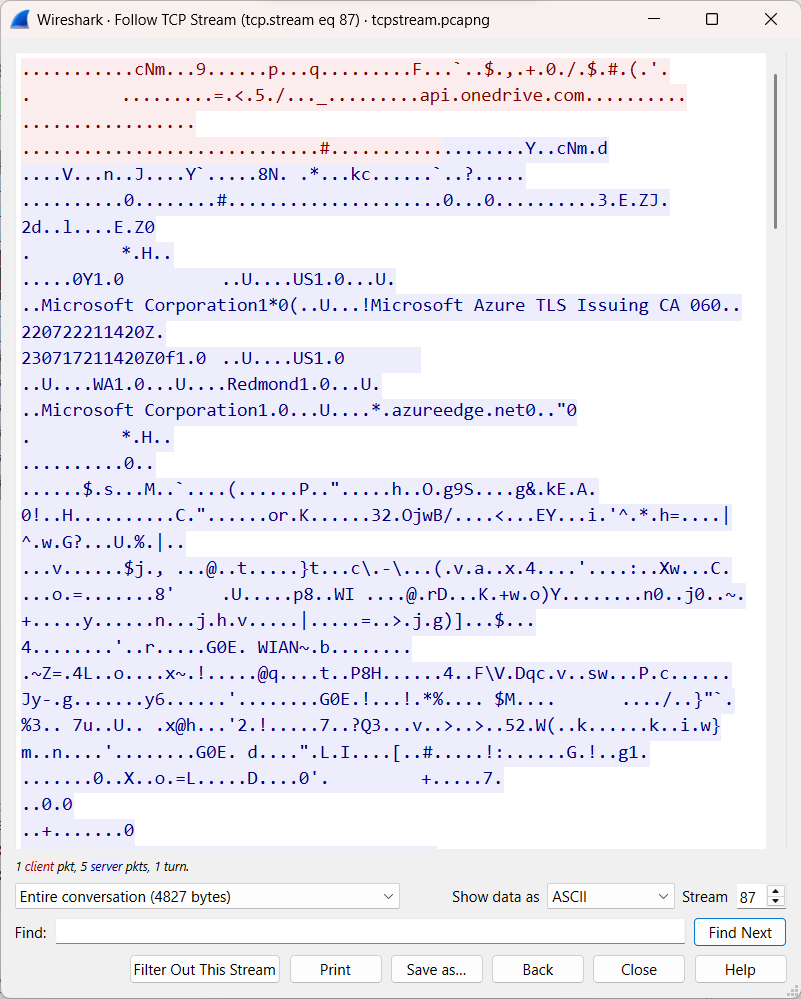
\includegraphics[width=0.4\textwidth]{stream.png}
\end{figure}

\subsection{协议分层统计}

以802.11为例,可以通过协议分层统计统计使用到了哪些协议,如图~\ref{fig:ph}。

可以发现所有的包都包含在802.11中。

\begin{figure}[htb]
	\centering
	\caption{协议分层统计}
	\label{fig:ph}
	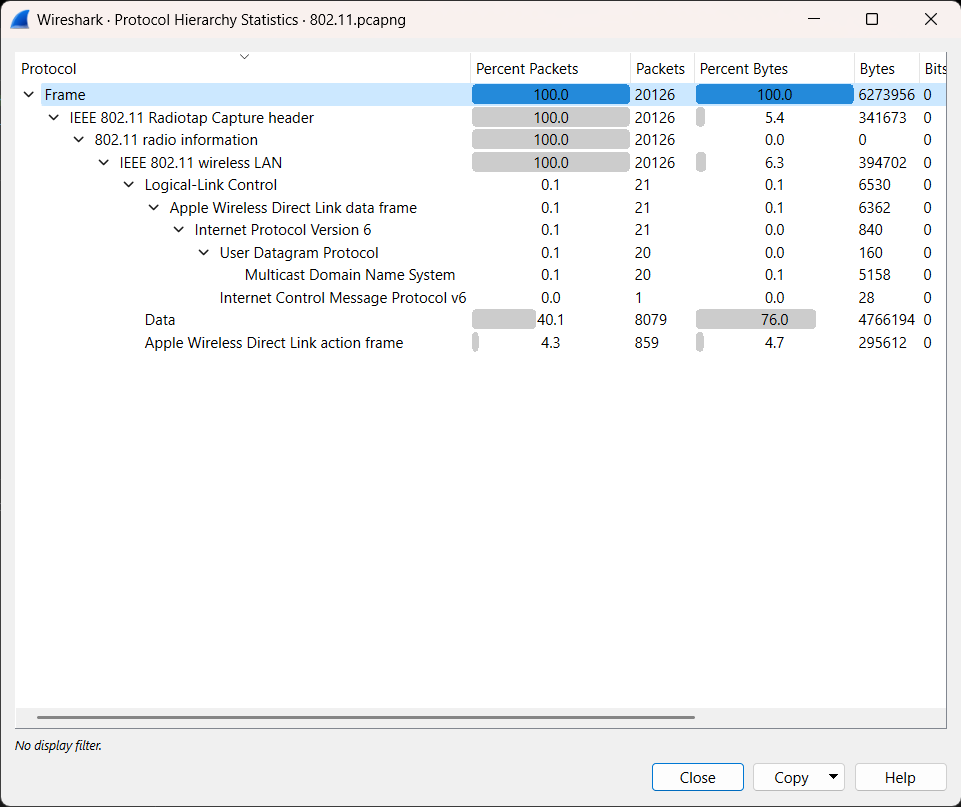
\includegraphics[width=0.4\textwidth]{ph.png}
\end{figure}

\end{spacing}

\end{document}